\documentclass{beamer}
\usepackage[utf8]{inputenc}

\usetheme{Madrid}
\usecolortheme{default}
\usepackage{amsmath,amssymb,amsfonts,amsthm}
\usepackage{txfonts}
\usepackage{tkz-euclide}
\usepackage{listings}
\usepackage{adjustbox}
\usepackage{array}
\usepackage{tabularx}
\usepackage{gvv}
\usepackage{lmodern}
\usepackage{circuitikz}
\usepackage{tikz}
\usepackage{graphicx}

\setbeamertemplate{page number in head/foot}[totalframenumber]

\usepackage{tcolorbox}
\tcbuselibrary{minted,breakable,xparse,skins}



\definecolor{bg}{gray}{0.95}
\DeclareTCBListing{mintedbox}{O{}m!O{}}{%
  breakable=true,
  listing engine=minted,
  listing only,
  minted language=#2,
  minted style=default,
  minted options={%
    linenos,
    gobble=0,
    breaklines=true,
    breakafter=,,
    fontsize=\small,
    numbersep=8pt,
    #1},
  boxsep=0pt,
  left skip=0pt,
  right skip=0pt,
  left=25pt,
  right=0pt,
  top=3pt,
  bottom=3pt,
  arc=5pt,
  leftrule=0pt,
  rightrule=0pt,
  bottomrule=2pt,
  toprule=2pt,
  colback=bg,
  colframe=orange!70,
  enhanced,
  overlay={%
    \begin{tcbclipinterior}
    \fill[orange!20!white] (frame.south west) rectangle ([xshift=20pt]frame.north west);
    \end{tcbclipinterior}},
  #3,
}
\lstset{
    language=C,
    basicstyle=\ttfamily\small,
    keywordstyle=\color{blue},
    stringstyle=\color{orange},
    commentstyle=\color{green!60!black},
    numbers=left,
    numberstyle=\tiny\color{gray},
    breaklines=true,
    showstringspaces=false,
}
%------------------------------------------------------------

\title
{2.10.23}
\author 
{AI25BTECH11034 - Sujal Chauhan }



\begin{document}

\frame{\titlepage}
\begin{frame}{Question}
Show that four points $\vec{A}(4,5,1)$, $\vec{B}(0,-1,-1)$, $\vec{C}(3,9,4)$, $\vec{D}(-4,4,4)$ are coplanar.




\end{frame}

\begin{frame}{Theory}
   If $N$ points in $\mathbb{R}^3$ are given as 
\[
X_i = (x_i, y_i, z_i), \quad i = 1,2,\dots,N,
\] 
Let equation of the given plane be 

all four point must satisfy the equation of plane 
\begin{align}
\myvec{\vec{A}&&\vec{B}&&\vec{C} && \vec{D}}=\vec{K}
\end{align}
Now equation will be 
\begin{align}
    \vec{K}^T\vec{n}=\myvec{1 \\ 1\\ 1\\ 1}
\end{align}
\end{frame}

\begin{frame}{Theory}
    

making augment matrix which is 

    \begin{align}
 \myvec{
x_1 & y_1 & z_1 & | & 1 \\
x_2 & y_2 & z_2 & | & 1 \\
x_3 & y_3 & z_3 & | & 1 \\
x_4 & y_4 & z_4 & | & 1
} 
\end{align}


then the condition for coplanarity is that the augmented matrix
\begin{align}
A = \myvec{
x_1 & y_1 & z_1 & 1 \\
x_2 & y_2 & z_2 & 1 \\
x_3& y_3 & z_3 & 1 \\
x_4 & y_4 & z_4 & 1
}
\end{align}
satisfies
\begin{align}
\operatorname{rank}(A) \leq 3.
\end{align}
\end{frame}


\begin{frame}{Solution}
Equation of plane:
\begin{align}
    \vec{n}^\top\vec{x}=1
\end{align}
Now we have:
Four point which satisfy the plane can be expressed as:
\begin{align}
    \myvec{4 && 5 && 1 \\
           0 && -1 && -1 \\
           3 && 9 && 4 \\
           -4 && 4 && 4 } \vec{n}=\myvec{1 \\ 1 \\ 1 \\1}      
\end{align}
Given augment matrix is :
\begin{align}
    \myvec{4 && 5 && 1 &|1\\
           0 && -1 && -1&|1 \\
           3 && 9 && 4 &|1\\
           -4 && 4 && 4 &|1}
\end{align}
\end{frame}
\begin{frame}{Solution}
    For the given four points to be coplanar, the rank of the following matrix must be less than 4:
\begin{align}
\mathbf{A}=\myvec{ 
4 & 5 & 1 & 1\\
0 & -1 & -1 & 1 \\
3 & 9 & 4 & 1\\
-4 & 4 & 4 & 1 
}
\end{align}

\begin{align}
&\xrightarrow{R_3 \to R_3 - \tfrac{3}{4}R_1,\; R_4 \to R_4 + R_1}
\myvec{
4 & 5 & 1 & 1 \\
0 & -1 & -1 & 1 \\
0 & \tfrac{21}{4} & \tfrac{13}{4} & \tfrac{1}{4} \\
0 & 9 & 5 & 2
}
\end{align}
\end{frame}
\begin{frame}{Solution}
\begin{align}
&\xrightarrow{R_1 \to \tfrac{1}{4}R_1}
\myvec{
1 & \tfrac{5}{4} & \tfrac{1}{4} & \tfrac{1}{4} \\
0 & -1 & -1 & 1 \\
0 & \tfrac{21}{4} & \tfrac{13}{4} & \tfrac{1}{4} \\
0 & 9 & 5 & 2
}
\end{align}

\begin{align}
&\xrightarrow{R_2 \to -R_2}
\myvec{
1 & \tfrac{5}{4} & \tfrac{1}{4} & \tfrac{1}{4} \\
0 & 1 & 1 & -1 \\
0 & \tfrac{21}{4} & \tfrac{13}{4} & \tfrac{1}{4} \\
0 & 9 & 5 & 2
}
\end{align}

\begin{align}
&\xrightarrow{R_3 \to R_3 - \tfrac{21}{4}R_2,\; R_4 \to R_4 - 9R_2}
\myvec{
1 & \tfrac{5}{4} & \tfrac{1}{4} & \tfrac{1}{4} \\
0 & 1 & 1 & -1 \\
0 & 0 & -2 & \tfrac{22}{4} \\
0 & 0 & -4 & 11
}
\end{align}
\end{frame}
\begin{frame}{Solution}
\begin{align}
&\xrightarrow{R_3 \to -\tfrac{1}{2}R_3}
\myvec{
1 & \tfrac{5}{4} & \tfrac{1}{4} & \tfrac{1}{4} \\
0 & 1 & 1 & -1 \\
0 & 0 & 1 & -\tfrac{11}{4} \\
0 & 0 & -4 & 11
}
\end{align}

\begin{align}
&\xrightarrow{R_4 \to R_4 + 4R_3}
\myvec{
1 & \tfrac{5}{4} & \tfrac{1}{4} & \tfrac{1}{4} \\
0 & 1 & 1 & -1 \\
0 & 0 & 1 & -\tfrac{11}{4} \\
0 & 0 & 0 & 0
}
\end{align}

Thus,
\begin{align}
\operatorname{rank}(\mathbf{A}) = 3 \;<\; 4 \;\;\implies\;\;
\text{The given points are coplanar.}
\end{align}
\end{frame}
\begin{frame}{figure}
\begin{figure}[H]
    \centering
    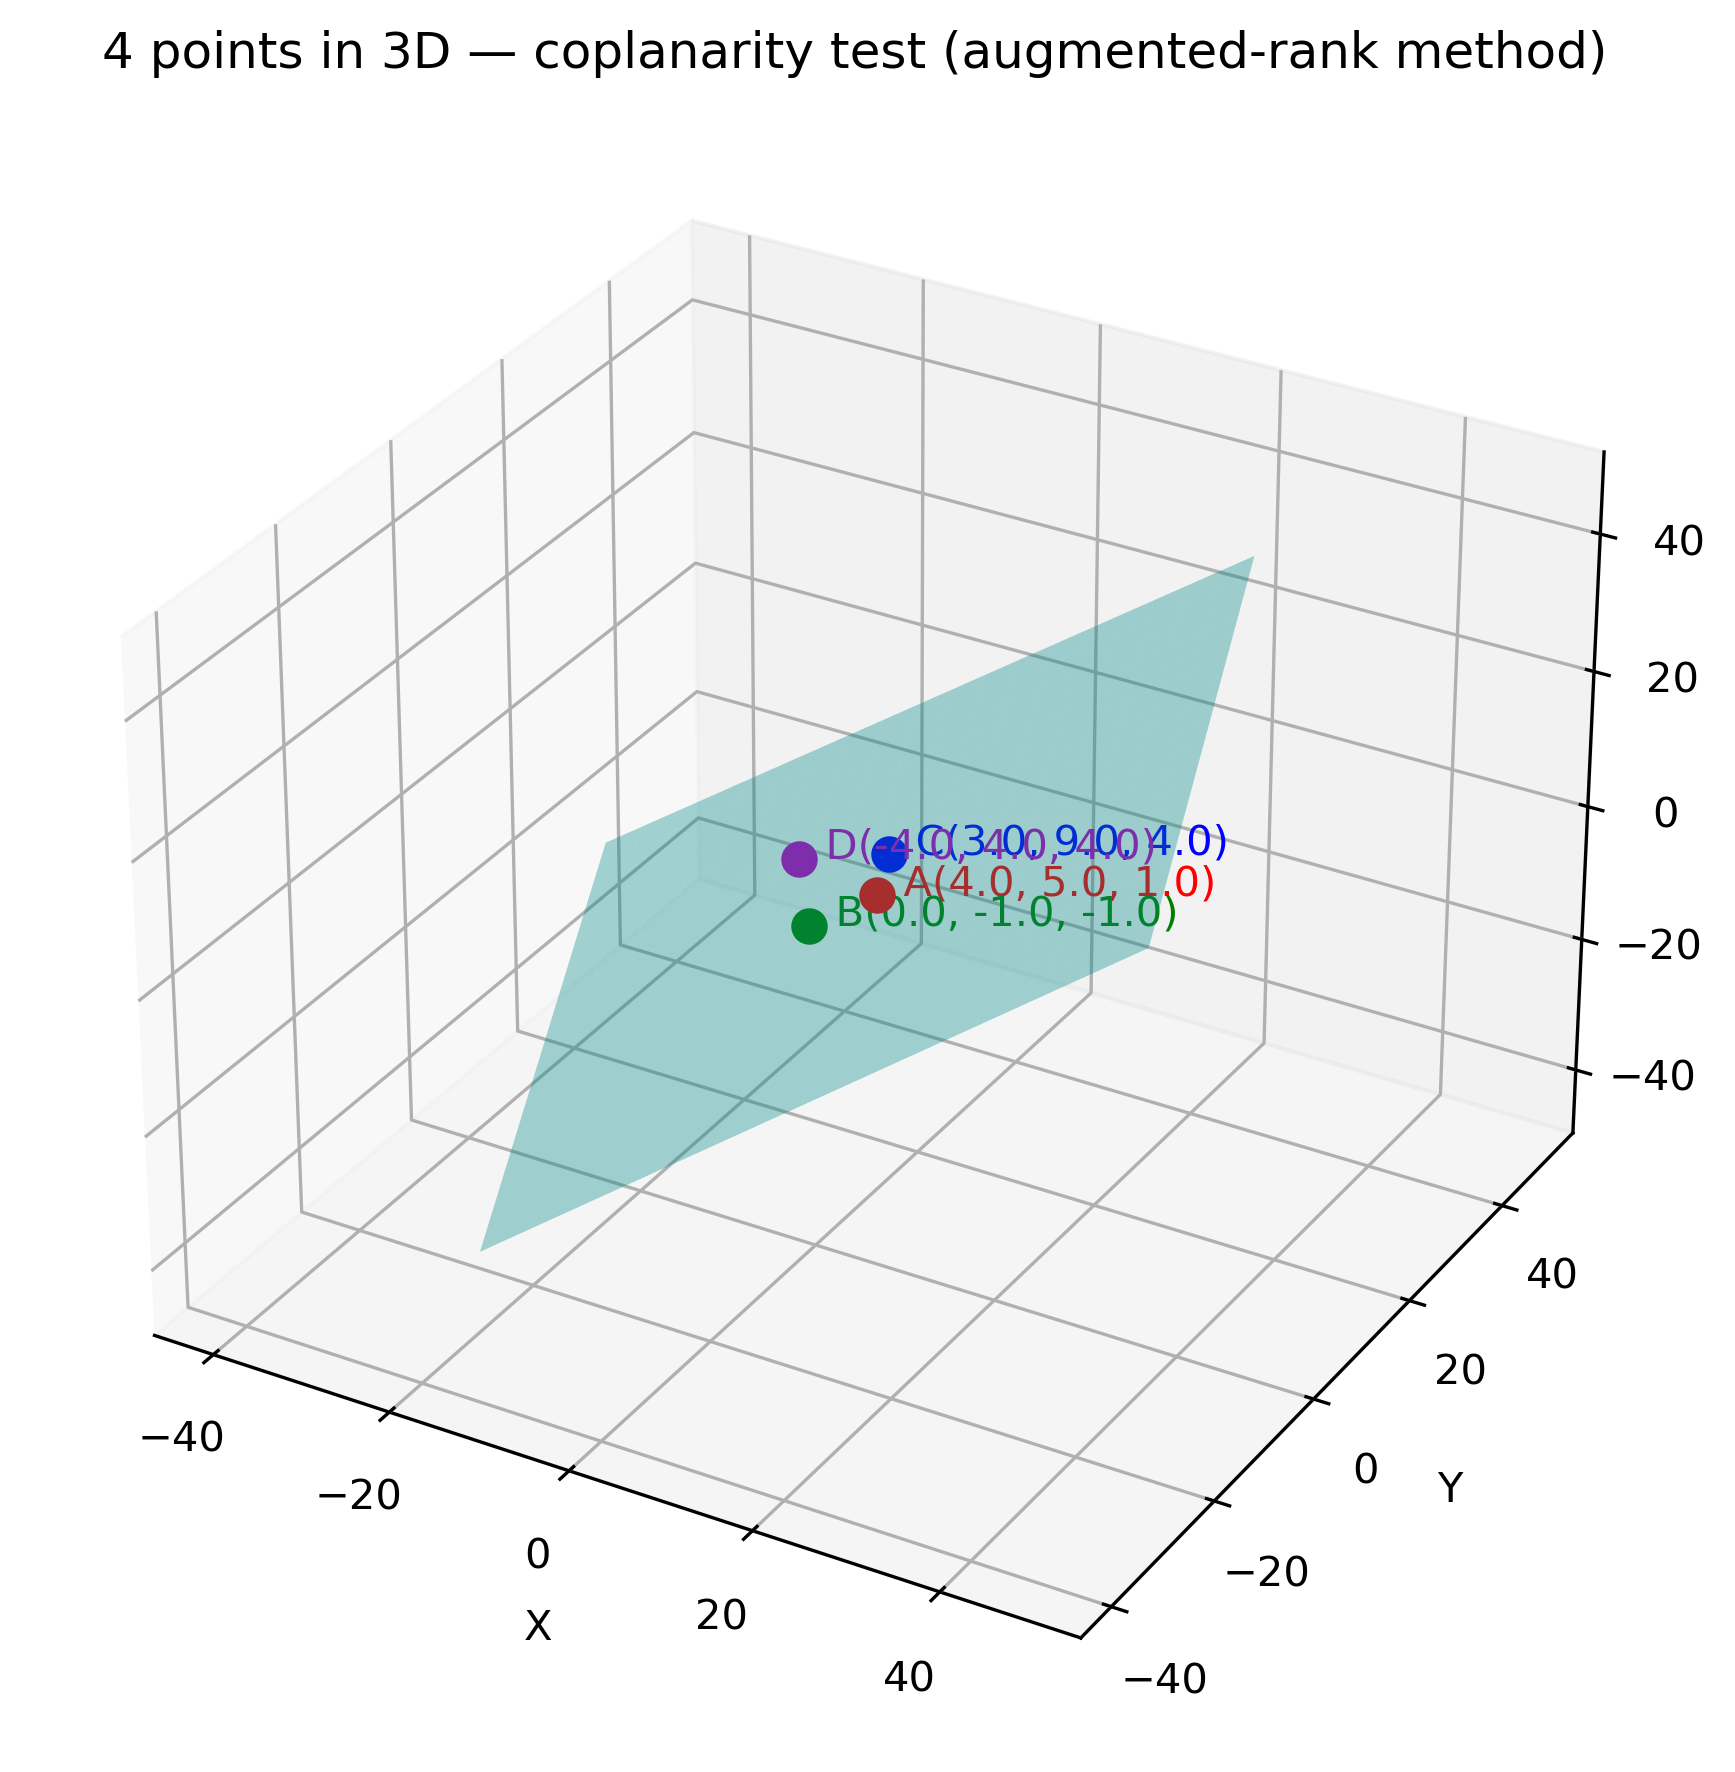
\includegraphics[width=0.45\linewidth]{figures/points_coplanarity.png}
    \caption{Geometric visualization of points $A, B, C, D$ lying on the same plane.}
    \label{fig:coplanarity}
\end{figure}    
\end{frame}



\end{document}
